\documentclass[twoside]{book}

% Packages required by doxygen
\usepackage{fixltx2e}
\usepackage{calc}
\usepackage{doxygen}
\usepackage{graphicx}
\usepackage[utf8]{inputenc}
\usepackage{makeidx}
\usepackage{multicol}
\usepackage{multirow}
\PassOptionsToPackage{warn}{textcomp}
\usepackage{textcomp}
\usepackage[nointegrals]{wasysym}
\usepackage[table]{xcolor}

% Font selection
\usepackage[T1]{fontenc}
\usepackage{mathptmx}
\usepackage[scaled=.90]{helvet}
\usepackage{courier}
\usepackage{amssymb}
\usepackage{sectsty}
\renewcommand{\familydefault}{\sfdefault}
\allsectionsfont{%
  \fontseries{bc}\selectfont%
  \color{darkgray}%
}
\renewcommand{\DoxyLabelFont}{%
  \fontseries{bc}\selectfont%
  \color{darkgray}%
}
\newcommand{\+}{\discretionary{\mbox{\scriptsize$\hookleftarrow$}}{}{}}

% Page & text layout
\usepackage{geometry}
\geometry{%
  a4paper,%
  top=2.5cm,%
  bottom=2.5cm,%
  left=2.5cm,%
  right=2.5cm%
}
\tolerance=750
\hfuzz=15pt
\hbadness=750
\setlength{\emergencystretch}{15pt}
\setlength{\parindent}{0cm}
\setlength{\parskip}{0.2cm}
\makeatletter
\renewcommand{\paragraph}{%
  \@startsection{paragraph}{4}{0ex}{-1.0ex}{1.0ex}{%
    \normalfont\normalsize\bfseries\SS@parafont%
  }%
}
\renewcommand{\subparagraph}{%
  \@startsection{subparagraph}{5}{0ex}{-1.0ex}{1.0ex}{%
    \normalfont\normalsize\bfseries\SS@subparafont%
  }%
}
\makeatother

% Headers & footers
\usepackage{fancyhdr}
\pagestyle{fancyplain}
\fancyhead[LE]{\fancyplain{}{\bfseries\thepage}}
\fancyhead[CE]{\fancyplain{}{}}
\fancyhead[RE]{\fancyplain{}{\bfseries\leftmark}}
\fancyhead[LO]{\fancyplain{}{\bfseries\rightmark}}
\fancyhead[CO]{\fancyplain{}{}}
\fancyhead[RO]{\fancyplain{}{\bfseries\thepage}}
\fancyfoot[LE]{\fancyplain{}{}}
\fancyfoot[CE]{\fancyplain{}{}}
\fancyfoot[RE]{\fancyplain{}{\bfseries\scriptsize Generated on Fri Nov 14 2014 14\+:15\+:48 for F\+B\+K\+V\+O\+Controller by Doxygen }}
\fancyfoot[LO]{\fancyplain{}{\bfseries\scriptsize Generated on Fri Nov 14 2014 14\+:15\+:48 for F\+B\+K\+V\+O\+Controller by Doxygen }}
\fancyfoot[CO]{\fancyplain{}{}}
\fancyfoot[RO]{\fancyplain{}{}}
\renewcommand{\footrulewidth}{0.4pt}
\renewcommand{\chaptermark}[1]{%
  \markboth{#1}{}%
}
\renewcommand{\sectionmark}[1]{%
  \markright{\thesection\ #1}%
}

% Indices & bibliography
\usepackage{natbib}
\usepackage[titles]{tocloft}
\setcounter{tocdepth}{3}
\setcounter{secnumdepth}{5}
\makeindex

% Hyperlinks (required, but should be loaded last)
\usepackage{ifpdf}
\ifpdf
  \usepackage[pdftex,pagebackref=true]{hyperref}
\else
  \usepackage[ps2pdf,pagebackref=true]{hyperref}
\fi
\hypersetup{%
  colorlinks=true,%
  linkcolor=blue,%
  citecolor=blue,%
  unicode%
}

% Custom commands
\newcommand{\clearemptydoublepage}{%
  \newpage{\pagestyle{empty}\cleardoublepage}%
}


%===== C O N T E N T S =====

\begin{document}

% Titlepage & ToC
\hypersetup{pageanchor=false,
             bookmarks=true,
             bookmarksnumbered=true,
             pdfencoding=unicode
            }
\pagenumbering{roman}
\begin{titlepage}
\vspace*{7cm}
\begin{center}%
{\Large F\+B\+K\+V\+O\+Controller }\\
\vspace*{1cm}
{\large Generated by Doxygen 1.8.8}\\
\vspace*{0.5cm}
{\small Fri Nov 14 2014 14:15:48}\\
\end{center}
\end{titlepage}
\clearemptydoublepage
\tableofcontents
\clearemptydoublepage
\pagenumbering{arabic}
\hypersetup{pageanchor=true}

%--- Begin generated contents ---
\chapter{Contributing}
\label{md__c_o_n_t_r_i_b_u_t_i_n_g}
\hypertarget{md__c_o_n_t_r_i_b_u_t_i_n_g}{}
We want to make contributing to K\+V\+O\+Controller as easy and transparent as possible. If you run into problems, please open an issue. We also actively welcome pull requests.

\subsection*{Pull Requests}


\begin{DoxyEnumerate}
\item Fork the repo and create your branch from {\ttfamily master}.
\item If you've added code that should be tested, add tests
\item If you've changed A\+P\+Is, update the documentation.
\item Ensure the test suite passes.
\item Make sure your code lints.
\item If you haven't already, complete the Contributor License Agreement (\char`\"{}\+C\+L\+A\char`\"{}).
\end{DoxyEnumerate}

\subsection*{Contributor License Agreement (\char`\"{}\+C\+L\+A\char`\"{})}

In order to accept your pull request, we need you to submit a C\+L\+A. You only need to do this once to work on any of Facebook's open source projects.

Complete your C\+L\+A here\+: \href{https://developers.facebook.com/opensource/cla}{\tt https\+://developers.\+facebook.\+com/opensource/cla}

\subsection*{Issues}

We use Git\+Hub issues to track public bugs. Please ensure your description is clear and has sufficient instructions to be able to reproduce the issue.

\subsection*{Coding Style}


\begin{DoxyItemize}
\item 2 spaces for indentation rather than tabs
\end{DoxyItemize}

\subsection*{License}

By contributing to K\+V\+O\+Controller, you agree that your contributions will be licensed under its B\+S\+D license. 
\chapter{\mbox{[}K\+V\+O\+Controller\mbox{]}(https\+://github.com/facebook/\+K\+V\+O\+Controller)}
\label{md__r_e_a_d_m_e}
\hypertarget{md__r_e_a_d_m_e}{}
\href{https://travis-ci.org/facebook/KVOController}{\tt !\mbox{[}Build Status\mbox{]}(https\+://travis-\/ci.\+org/facebook/\+K\+V\+O\+Controller.\+png?branch=master)} \href{http://cocoadocs.org/docsets/KVOController}{\tt !\mbox{[}Version\mbox{]}(https\+://cocoapod-\/badges.\+herokuapp.\+com/v/\+K\+V\+O\+Controller/badge.\+png)} \href{http://cocoadocs.org/docsets/KVOController}{\tt !\mbox{[}Platform\mbox{]}(https\+://cocoapod-\/badges.\+herokuapp.\+com/p/\+K\+V\+O\+Controller/badge.\+png)}

Key-\/value observing is a particularly useful technique for communicating between layers in a Model-\/\+View-\/\+Controller application. K\+V\+O\+Controller builds on Cocoa's time-\/tested key-\/value observing implementation. It offers a simple, modern A\+P\+I, that is also thread safe. Benefits include\+:


\begin{DoxyItemize}
\item Notification using blocks, custom actions, or N\+S\+Key\+Value\+Observing callback.
\item No exceptions on observer removal.
\item Implicit observer removal on controller dealloc.
\item Thread-\/safety with special guards against observer resurrection – \href{http://openradar.appspot.com/radar?id=5305010728468480}{\tt rdar\+://15985376}.
\end{DoxyItemize}

For more information on K\+V\+O, see Apple's \href{https://developer.apple.com/library/mac/documentation/Cocoa/Conceptual/KeyValueObserving/KeyValueObserving.html}{\tt Introduction to Key-\/\+Value Observing}.

\subsection*{Usage}

Example apps for i\+O\+S and O\+S X are included with the project. Here is one simple usage pattern\+:

```objective-\/c // create K\+V\+O controller with observer \hyperlink{interface_f_b_k_v_o_controller}{F\+B\+K\+V\+O\+Controller} $\ast$\+K\+V\+O\+Controller = \mbox{[}\hyperlink{interface_f_b_k_v_o_controller}{F\+B\+K\+V\+O\+Controller} controller\+With\+Observer\+:self\mbox{]}; self.\+K\+V\+O\+Controller = K\+V\+O\+Controller;

// observe clock date property \mbox{[}self.\+K\+V\+O\+Controller observe\+:clock key\+Path\+:"date" options\+:N\+S\+Key\+Value\+Observing\+Option\+Initial$\vert$\+N\+S\+Key\+Value\+Observing\+Option\+New block\+:$^\wedge$(Clock\+View $\ast$clock\+View, Clock $\ast$clock, N\+S\+Dictionary $\ast$change) \{

// update clock view with new value clock\+View.\+date = change\mbox{[}N\+S\+Key\+Value\+Change\+New\+Key\mbox{]}; \}\mbox{]}; ```

While simple, the above example is complete. A clock view creates a K\+V\+O controller to observe the clock date property. A block callback is used to handle initial and change notification. Unobservation happens implicitly on controller deallocation, since a strong reference to the {\ttfamily K\+V\+O\+Controller} is kept.

Note\+: the observer specified must support weak references. The zeroing weak reference guards against notification of a deallocated observer instance.

\paragraph*{N\+S\+Object Category}

For an even easier usage, just {\ttfamily \#import $<$K\+V\+O\+Controller/\+N\+S\+Object+\+F\+B\+K\+V\+O\+Controller.h} for an automatic {\ttfamily K\+V\+O\+Controller} property on all objects.

```objc \mbox{[}self.\+K\+V\+O\+Controller observe\+:clock key\+Path\+:"date" options\+:N\+S\+Key\+Value\+Observing\+Option\+Initial$\vert$\+N\+S\+Key\+Value\+Observing\+Option\+New action\+:(update\+Clock\+With\+Date\+Change\+:)\mbox{]}; ```

\subsection*{Prerequisites}

K\+V\+O\+Controller takes advantage of recent Objective-\/\+C runtime advances, including A\+R\+C and weak collections. It requires\+:


\begin{DoxyItemize}
\item i\+O\+S 6 or later.
\item O\+S X 10.\+7 or later.
\end{DoxyItemize}

\subsection*{Installation}

To install using Cocoa\+Pods, add the following to your project Podfile\+:

```ruby pod 'K\+V\+O\+Controller' ```

Alternatively, drag and drop \hyperlink{_f_b_k_v_o_controller_8h_source}{F\+B\+K\+V\+O\+Controller.\+h} and F\+B\+K\+V\+O\+Controller.\+m into your Xcode project, agreeing to copy files if needed. For i\+O\+S applications, you can choose to link against the static library target of the K\+V\+O\+Controller project.

Having installed using Cocoa\+Pods, add the following to import in Objective-\/\+C\+: ```objective-\/c \#import $<$\hyperlink{_f_b_k_v_o_controller_8h_source}{K\+V\+O\+Controller/\+F\+B\+K\+V\+O\+Controller.\+h}$>$ ```

\subsection*{Testing}

The unit tests included use Cocoa\+Pods for managing dependencies. Install Cocoa\+Pods if you haven't already done so. Then, at the command line, navigate to the root K\+V\+O\+Controller directory and type\+:

```sh pod install ```

This will install and add test dependencies on O\+C\+Hamcrest and O\+C\+Mockito. Re-\/open the Xcode K\+V\+O\+Controller workspace and Test, ⌘\+U.

\subsection*{Licence}

K\+V\+O\+Controller is released under a B\+S\+D License. See L\+I\+C\+E\+N\+S\+E file for details. 
\chapter{Hierarchical Index}
\section{Class Hierarchy}
This inheritance list is sorted roughly, but not completely, alphabetically\+:\begin{DoxyCompactList}
\item N\+S\+Object\begin{DoxyCompactList}
\item \contentsline{section}{\+\_\+\+F\+B\+K\+V\+O\+Info}{\pageref{interface___f_b_k_v_o_info}}{}
\item \contentsline{section}{\+\_\+\+F\+B\+K\+V\+O\+Shared\+Controller}{\pageref{interface___f_b_k_v_o_shared_controller}}{}
\item \contentsline{section}{F\+B\+K\+V\+O\+Controller}{\pageref{interface_f_b_k_v_o_controller}}{}
\end{DoxyCompactList}
\item \contentsline{section}{N\+S\+Object(F\+B\+K\+V\+O\+Controller)}{\pageref{category_n_s_object_07_f_b_k_v_o_controller_08}}{}
\end{DoxyCompactList}

\chapter{Class Index}
\section{Class List}
Here are the classes, structs, unions and interfaces with brief descriptions\+:\begin{DoxyCompactList}
\item\contentsline{section}{\hyperlink{interface___f_b_k_v_o_info}{\+\_\+\+F\+B\+K\+V\+O\+Info} }{\pageref{interface___f_b_k_v_o_info}}{}
\item\contentsline{section}{\hyperlink{interface___f_b_k_v_o_shared_controller}{\+\_\+\+F\+B\+K\+V\+O\+Shared\+Controller} }{\pageref{interface___f_b_k_v_o_shared_controller}}{}
\item\contentsline{section}{\hyperlink{interface_f_b_k_v_o_controller}{F\+B\+K\+V\+O\+Controller} }{\pageref{interface_f_b_k_v_o_controller}}{}
\item\contentsline{section}{\hyperlink{category_n_s_object_07_f_b_k_v_o_controller_08}{N\+S\+Object(\+F\+B\+K\+V\+O\+Controller)} \\*\+: }{\pageref{category_n_s_object_07_f_b_k_v_o_controller_08}}{}
\end{DoxyCompactList}

\chapter{Class Documentation}
\hypertarget{interface___f_b_k_v_o_info}{\section{\+\_\+\+F\+B\+K\+V\+O\+Info Class Reference}
\label{interface___f_b_k_v_o_info}\index{\+\_\+\+F\+B\+K\+V\+O\+Info@{\+\_\+\+F\+B\+K\+V\+O\+Info}}
}
Inheritance diagram for \+\_\+\+F\+B\+K\+V\+O\+Info\+:\begin{figure}[H]
\begin{center}
\leavevmode
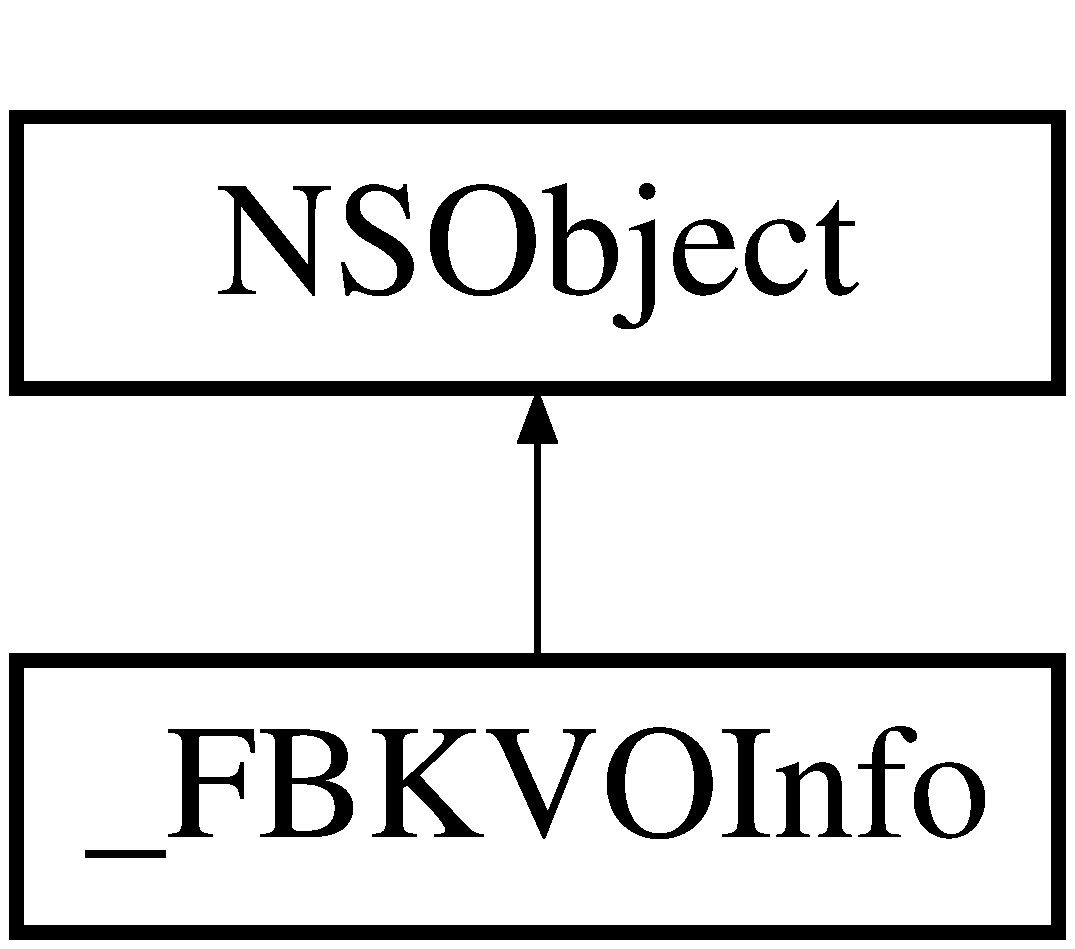
\includegraphics[height=2.000000cm]{interface___f_b_k_v_o_info}
\end{center}
\end{figure}


\subsection{Detailed Description}
The key-\/value observation info.  Object equality is only used within the scope of a controller instance. Safely omit controller from equality definition. 

The documentation for this class was generated from the following file\+:\begin{DoxyCompactItemize}
\item 
F\+B\+K\+V\+O\+Controller/F\+B\+K\+V\+O\+Controller.\+m\end{DoxyCompactItemize}

\hypertarget{interface___f_b_k_v_o_shared_controller}{\section{\+\_\+\+F\+B\+K\+V\+O\+Shared\+Controller Class Reference}
\label{interface___f_b_k_v_o_shared_controller}\index{\+\_\+\+F\+B\+K\+V\+O\+Shared\+Controller@{\+\_\+\+F\+B\+K\+V\+O\+Shared\+Controller}}
}
Inheritance diagram for \+\_\+\+F\+B\+K\+V\+O\+Shared\+Controller\+:\begin{figure}[H]
\begin{center}
\leavevmode
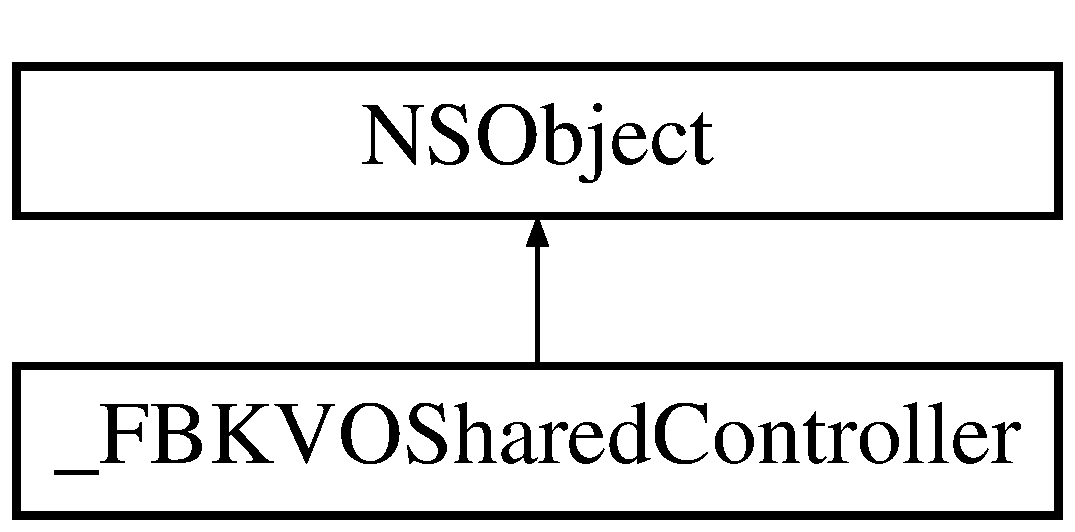
\includegraphics[height=2.000000cm]{interface___f_b_k_v_o_shared_controller}
\end{center}
\end{figure}
\subsection*{Instance Methods}
\begin{DoxyCompactItemize}
\item 
(void) -\/ \hyperlink{interface___f_b_k_v_o_shared_controller_a3c86b19c63b309078c372d3ba9c82423}{observe\+:info\+:}
\item 
(void) -\/ \hyperlink{interface___f_b_k_v_o_shared_controller_a8c1ecb634733652d00e1d0171eea4856}{unobserve\+:info\+:}
\item 
(void) -\/ \hyperlink{interface___f_b_k_v_o_shared_controller_a672c0e721f004e5f34ea8e497d9f4841}{unobserve\+:infos\+:}
\end{DoxyCompactItemize}
\subsection*{Class Methods}
\begin{DoxyCompactItemize}
\item 
(instancetype) + \hyperlink{interface___f_b_k_v_o_shared_controller_afc8dc49222e1a694297251398e1a5341}{shared\+Controller}
\end{DoxyCompactItemize}


\subsection{Detailed Description}
The shared K\+V\+O controller instance.  Acts as a receptionist, receiving and forwarding K\+V\+O notifications. 

\subsection{Method Documentation}
\hypertarget{interface___f_b_k_v_o_shared_controller_a3c86b19c63b309078c372d3ba9c82423}{\index{\+\_\+\+F\+B\+K\+V\+O\+Shared\+Controller@{\+\_\+\+F\+B\+K\+V\+O\+Shared\+Controller}!observe\+:info\+:@{observe\+:info\+:}}
\index{observe\+:info\+:@{observe\+:info\+:}!\+\_\+\+F\+B\+K\+V\+O\+Shared\+Controller@{\+\_\+\+F\+B\+K\+V\+O\+Shared\+Controller}}
\subsubsection[{observe\+:info\+:}]{\setlength{\rightskip}{0pt plus 5cm}-\/ (void) observe\+: 
\begin{DoxyParamCaption}
\item[{(id)}]{object}
\item[{info:({\bf \+\_\+\+F\+B\+K\+V\+O\+Info}$\ast$)}]{info}
\end{DoxyParamCaption}
}}\label{interface___f_b_k_v_o_shared_controller_a3c86b19c63b309078c372d3ba9c82423}
observe an object, info pair \hypertarget{interface___f_b_k_v_o_shared_controller_afc8dc49222e1a694297251398e1a5341}{\index{\+\_\+\+F\+B\+K\+V\+O\+Shared\+Controller@{\+\_\+\+F\+B\+K\+V\+O\+Shared\+Controller}!shared\+Controller@{shared\+Controller}}
\index{shared\+Controller@{shared\+Controller}!\+\_\+\+F\+B\+K\+V\+O\+Shared\+Controller@{\+\_\+\+F\+B\+K\+V\+O\+Shared\+Controller}}
\subsubsection[{shared\+Controller}]{\setlength{\rightskip}{0pt plus 5cm}+ (instancetype) shared\+Controller 
\begin{DoxyParamCaption}
{}
\end{DoxyParamCaption}
}}\label{interface___f_b_k_v_o_shared_controller_afc8dc49222e1a694297251398e1a5341}
A shared instance that never deallocates. \hypertarget{interface___f_b_k_v_o_shared_controller_a8c1ecb634733652d00e1d0171eea4856}{\index{\+\_\+\+F\+B\+K\+V\+O\+Shared\+Controller@{\+\_\+\+F\+B\+K\+V\+O\+Shared\+Controller}!unobserve\+:info\+:@{unobserve\+:info\+:}}
\index{unobserve\+:info\+:@{unobserve\+:info\+:}!\+\_\+\+F\+B\+K\+V\+O\+Shared\+Controller@{\+\_\+\+F\+B\+K\+V\+O\+Shared\+Controller}}
\subsubsection[{unobserve\+:info\+:}]{\setlength{\rightskip}{0pt plus 5cm}-\/ (void) unobserve\+: 
\begin{DoxyParamCaption}
\item[{(id)}]{object}
\item[{info:({\bf \+\_\+\+F\+B\+K\+V\+O\+Info} $\ast$)}]{info}
\end{DoxyParamCaption}
}}\label{interface___f_b_k_v_o_shared_controller_a8c1ecb634733652d00e1d0171eea4856}
unobserve an object, info pair \hypertarget{interface___f_b_k_v_o_shared_controller_a672c0e721f004e5f34ea8e497d9f4841}{\index{\+\_\+\+F\+B\+K\+V\+O\+Shared\+Controller@{\+\_\+\+F\+B\+K\+V\+O\+Shared\+Controller}!unobserve\+:infos\+:@{unobserve\+:infos\+:}}
\index{unobserve\+:infos\+:@{unobserve\+:infos\+:}!\+\_\+\+F\+B\+K\+V\+O\+Shared\+Controller@{\+\_\+\+F\+B\+K\+V\+O\+Shared\+Controller}}
\subsubsection[{unobserve\+:infos\+:}]{\setlength{\rightskip}{0pt plus 5cm}-\/ (void) unobserve\+: 
\begin{DoxyParamCaption}
\item[{(id)}]{object}
\item[{infos:(N\+S\+Set $\ast$)}]{infos}
\end{DoxyParamCaption}
}}\label{interface___f_b_k_v_o_shared_controller_a672c0e721f004e5f34ea8e497d9f4841}
unobserve an object with a set of infos 

The documentation for this class was generated from the following file\+:\begin{DoxyCompactItemize}
\item 
F\+B\+K\+V\+O\+Controller/F\+B\+K\+V\+O\+Controller.\+m\end{DoxyCompactItemize}

\hypertarget{interface_f_b_k_v_o_controller}{\section{F\+B\+K\+V\+O\+Controller Class Reference}
\label{interface_f_b_k_v_o_controller}\index{F\+B\+K\+V\+O\+Controller@{F\+B\+K\+V\+O\+Controller}}
}


{\ttfamily \#import $<$F\+B\+K\+V\+O\+Controller.\+h$>$}

Inheritance diagram for F\+B\+K\+V\+O\+Controller\+:\begin{figure}[H]
\begin{center}
\leavevmode
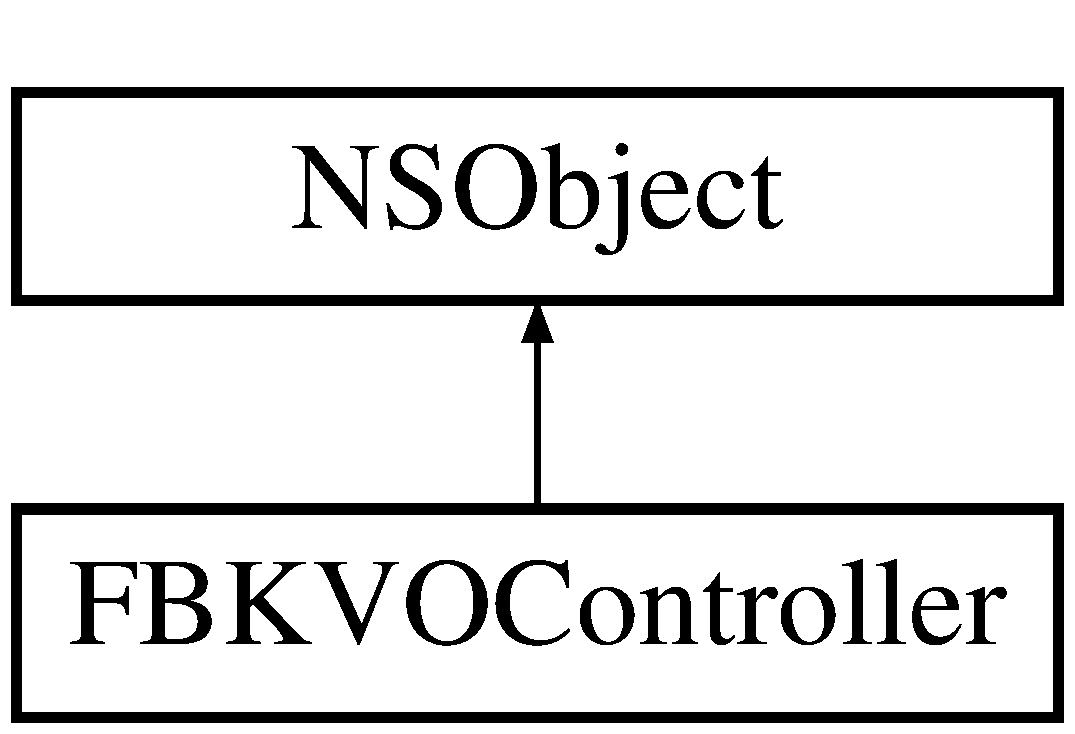
\includegraphics[height=2.000000cm]{interface_f_b_k_v_o_controller}
\end{center}
\end{figure}
\subsection*{Instance Methods}
\begin{DoxyCompactItemize}
\item 
(instancetype) -\/ \hyperlink{interface_f_b_k_v_o_controller_ab10c2daadcd69117b6dfddcdda0ca231}{init\+With\+Observer\+:retain\+Observed\+:}
\item 
(instancetype) -\/ \hyperlink{interface_f_b_k_v_o_controller_a0614e1c3de86e47a152cdf23aad5f85e}{init\+With\+Observer\+:}
\item 
(void) -\/ \hyperlink{interface_f_b_k_v_o_controller_a5e947c609b39d2e05dbf9e9e0639d1d4}{observe\+:key\+Path\+:options\+:block\+:}
\item 
(void) -\/ \hyperlink{interface_f_b_k_v_o_controller_a4558dee863033be98d3d59a16621edee}{observe\+:key\+Path\+:options\+:action\+:}
\item 
(void) -\/ \hyperlink{interface_f_b_k_v_o_controller_a09c725ec7fa8e649b3a1c2e5ecd004ae}{observe\+:key\+Path\+:options\+:context\+:}
\item 
(void) -\/ \hyperlink{interface_f_b_k_v_o_controller_a78b2d28e3b4bc208053a8d53c596f394}{observe\+:key\+Paths\+:options\+:block\+:}
\item 
(void) -\/ \hyperlink{interface_f_b_k_v_o_controller_a95f73613e406f372bf34906f56e89f4d}{observe\+:key\+Paths\+:options\+:action\+:}
\item 
(void) -\/ \hyperlink{interface_f_b_k_v_o_controller_a322a647907eebd55c01d185622e7ad39}{observe\+:key\+Paths\+:options\+:context\+:}
\item 
(void) -\/ \hyperlink{interface_f_b_k_v_o_controller_aebaeb37fe373939c8254984bdf3c518a}{unobserve\+:key\+Path\+:}
\item 
(void) -\/ \hyperlink{interface_f_b_k_v_o_controller_ae614819487de82c3a513610031834a6d}{unobserve\+:}
\item 
(void) -\/ \hyperlink{interface_f_b_k_v_o_controller_a68986621c451e29b46b6b8eda62e188e}{unobserve\+All}
\end{DoxyCompactItemize}
\subsection*{Class Methods}
\begin{DoxyCompactItemize}
\item 
(instancetype) + \hyperlink{interface_f_b_k_v_o_controller_ab8b4b15ecd54384a02f19db9fc284176}{controller\+With\+Observer\+:}
\end{DoxyCompactItemize}
\subsection*{Properties}
\begin{DoxyCompactItemize}
\item 
\hypertarget{interface_f_b_k_v_o_controller_a9a41b9bcda267b904af88265fa4c3611}{id \hyperlink{interface_f_b_k_v_o_controller_a9a41b9bcda267b904af88265fa4c3611}{observer}}\label{interface_f_b_k_v_o_controller_a9a41b9bcda267b904af88265fa4c3611}

\begin{DoxyCompactList}\small\item\em The observer notified on key-\/value change. Specified on initialization. \end{DoxyCompactList}\end{DoxyCompactItemize}


\subsection{Detailed Description}
\hyperlink{interface_f_b_k_v_o_controller}{F\+B\+K\+V\+O\+Controller} makes Key-\/\+Value Observing simpler and safer.  \hyperlink{interface_f_b_k_v_o_controller}{F\+B\+K\+V\+O\+Controller} adds support for handling key-\/value changes with blocks and custom actions, as well as the N\+S\+Key\+Value\+Observing callback. Notification will never message a deallocated observer. Observer removal never throws exceptions, and observers are removed implicitly on controller deallocation. \hyperlink{interface_f_b_k_v_o_controller}{F\+B\+K\+V\+O\+Controller} is also thread safe. When used in a concurrent environment, it protects observers from possible resurrection and avoids ensuing crash. By default, the controller maintains a strong reference to objects observed. 

\subsection{Method Documentation}
\hypertarget{interface_f_b_k_v_o_controller_ab8b4b15ecd54384a02f19db9fc284176}{\index{F\+B\+K\+V\+O\+Controller@{F\+B\+K\+V\+O\+Controller}!controller\+With\+Observer\+:@{controller\+With\+Observer\+:}}
\index{controller\+With\+Observer\+:@{controller\+With\+Observer\+:}!F\+B\+K\+V\+O\+Controller@{F\+B\+K\+V\+O\+Controller}}
\subsubsection[{controller\+With\+Observer\+:}]{\setlength{\rightskip}{0pt plus 5cm}+ (instancetype) controller\+With\+Observer\+: 
\begin{DoxyParamCaption}
\item[{(id)}]{\+\_\+\+Observer}
\end{DoxyParamCaption}
}}\label{interface_f_b_k_v_o_controller_ab8b4b15ecd54384a02f19db9fc284176}
Creates and returns an initialized K\+V\+O controller instance. 
\begin{DoxyParams}{Parameters}
{\em observer} & The object notified on key-\/value change. \\
\hline
\end{DoxyParams}
\begin{DoxyReturn}{Returns}
The initialized K\+V\+O controller instance. 
\end{DoxyReturn}
\hypertarget{interface_f_b_k_v_o_controller_a0614e1c3de86e47a152cdf23aad5f85e}{\index{F\+B\+K\+V\+O\+Controller@{F\+B\+K\+V\+O\+Controller}!init\+With\+Observer\+:@{init\+With\+Observer\+:}}
\index{init\+With\+Observer\+:@{init\+With\+Observer\+:}!F\+B\+K\+V\+O\+Controller@{F\+B\+K\+V\+O\+Controller}}
\subsubsection[{init\+With\+Observer\+:}]{\setlength{\rightskip}{0pt plus 5cm}-\/ (instancetype) init\+With\+Observer\+: 
\begin{DoxyParamCaption}
\item[{(id)}]{\+\_\+\+Observer}
\end{DoxyParamCaption}
}}\label{interface_f_b_k_v_o_controller_a0614e1c3de86e47a152cdf23aad5f85e}
Convenience initializer. 
\begin{DoxyParams}{Parameters}
{\em bserver} & The object notified on key-\/value change. The specified observer must support weak references. \\
\hline
\end{DoxyParams}
\begin{DoxyReturn}{Returns}
The initialized K\+V\+O controller instance.  By default, K\+V\+O controller retains objects observed. 
\end{DoxyReturn}
\hypertarget{interface_f_b_k_v_o_controller_ab10c2daadcd69117b6dfddcdda0ca231}{\index{F\+B\+K\+V\+O\+Controller@{F\+B\+K\+V\+O\+Controller}!init\+With\+Observer\+:retain\+Observed\+:@{init\+With\+Observer\+:retain\+Observed\+:}}
\index{init\+With\+Observer\+:retain\+Observed\+:@{init\+With\+Observer\+:retain\+Observed\+:}!F\+B\+K\+V\+O\+Controller@{F\+B\+K\+V\+O\+Controller}}
\subsubsection[{init\+With\+Observer\+:retain\+Observed\+:}]{\setlength{\rightskip}{0pt plus 5cm}-\/ (instancetype) {\bf init\+With\+Observer\+:} 
\begin{DoxyParamCaption}
\item[{(id)}]{\+\_\+\+Observer}
\item[{retainObserved:(B\+O\+O\+L)}]{\+\_\+\+Retain\+Observed}
\end{DoxyParamCaption}
}}\label{interface_f_b_k_v_o_controller_ab10c2daadcd69117b6dfddcdda0ca231}
The designated initializer. 
\begin{DoxyParams}{Parameters}
{\em observer} & The object notified on key-\/value change. The specified observer must support weak references. \\
\hline
{\em retain\+Observed} & Flag indicating whether observed objects should be retained. \\
\hline
\end{DoxyParams}
\begin{DoxyReturn}{Returns}
The initialized K\+V\+O controller instance.  Use retain\+Observed = N\+O when a strong reference between controller and observee would create a retain loop. When not retaining observees, special care must be taken to remove observation info prior to observee dealloc. 
\end{DoxyReturn}
\hypertarget{interface_f_b_k_v_o_controller_a4558dee863033be98d3d59a16621edee}{\index{F\+B\+K\+V\+O\+Controller@{F\+B\+K\+V\+O\+Controller}!observe\+:key\+Path\+:options\+:action\+:@{observe\+:key\+Path\+:options\+:action\+:}}
\index{observe\+:key\+Path\+:options\+:action\+:@{observe\+:key\+Path\+:options\+:action\+:}!F\+B\+K\+V\+O\+Controller@{F\+B\+K\+V\+O\+Controller}}
\subsubsection[{observe\+:key\+Path\+:options\+:action\+:}]{\setlength{\rightskip}{0pt plus 5cm}-\/ (void) observe\+: 
\begin{DoxyParamCaption}
\item[{(id)}]{object}
\item[{keyPath:(N\+S\+String $\ast$)}]{key\+Path}
\item[{options:(N\+S\+Key\+Value\+Observing\+Options)}]{options}
\item[{action:(S\+E\+L)}]{action}
\end{DoxyParamCaption}
}}\label{interface_f_b_k_v_o_controller_a4558dee863033be98d3d59a16621edee}
Registers observer for key-\/value change notification. 
\begin{DoxyParams}{Parameters}
{\em object} & The object to observe. \\
\hline
{\em key\+Path} & The key path to observe. \\
\hline
{\em options} & The N\+S\+Key\+Value\+Observing\+Options to use for observation. \\
\hline
{\em action} & The observer selector called on key-\/value change.  On key-\/value change, the observer's action selector is called. The selector provided should take the form of -\/property\+Did\+Change, -\/property\+Did\+Change\+: or -\/property\+Did\+Change\+:object\+:, where optional parameters delivered will be K\+V\+O change dictionary and object observed. Observing nil or observing an already observed object's key path results in no operation. \\
\hline
\end{DoxyParams}
\hypertarget{interface_f_b_k_v_o_controller_a5e947c609b39d2e05dbf9e9e0639d1d4}{\index{F\+B\+K\+V\+O\+Controller@{F\+B\+K\+V\+O\+Controller}!observe\+:key\+Path\+:options\+:block\+:@{observe\+:key\+Path\+:options\+:block\+:}}
\index{observe\+:key\+Path\+:options\+:block\+:@{observe\+:key\+Path\+:options\+:block\+:}!F\+B\+K\+V\+O\+Controller@{F\+B\+K\+V\+O\+Controller}}
\subsubsection[{observe\+:key\+Path\+:options\+:block\+:}]{\setlength{\rightskip}{0pt plus 5cm}-\/ (void) observe\+: 
\begin{DoxyParamCaption}
\item[{(id)}]{object}
\item[{keyPath:(N\+S\+String $\ast$)}]{key\+Path}
\item[{options:(N\+S\+Key\+Value\+Observing\+Options)}]{options}
\item[{block:(F\+B\+K\+V\+O\+Notification\+Block)}]{block}
\end{DoxyParamCaption}
}}\label{interface_f_b_k_v_o_controller_a5e947c609b39d2e05dbf9e9e0639d1d4}
Registers observer for key-\/value change notification. 
\begin{DoxyParams}{Parameters}
{\em object} & The object to observe. \\
\hline
{\em key\+Path} & The key path to observe. \\
\hline
{\em options} & The N\+S\+Key\+Value\+Observing\+Options to use for observation. \\
\hline
{\em block} & The block to execute on notification.  On key-\/value change, the specified block is called. Inorder to avoid retain loops, the block must avoid referencing the K\+V\+O controller or an owner thereof. Observing an already observed object key path or nil results in no operation. \\
\hline
\end{DoxyParams}
\hypertarget{interface_f_b_k_v_o_controller_a09c725ec7fa8e649b3a1c2e5ecd004ae}{\index{F\+B\+K\+V\+O\+Controller@{F\+B\+K\+V\+O\+Controller}!observe\+:key\+Path\+:options\+:context\+:@{observe\+:key\+Path\+:options\+:context\+:}}
\index{observe\+:key\+Path\+:options\+:context\+:@{observe\+:key\+Path\+:options\+:context\+:}!F\+B\+K\+V\+O\+Controller@{F\+B\+K\+V\+O\+Controller}}
\subsubsection[{observe\+:key\+Path\+:options\+:context\+:}]{\setlength{\rightskip}{0pt plus 5cm}-\/ (void) observe\+: 
\begin{DoxyParamCaption}
\item[{(id)}]{object}
\item[{keyPath:(N\+S\+String $\ast$)}]{key\+Path}
\item[{options:(N\+S\+Key\+Value\+Observing\+Options)}]{options}
\item[{context:(void $\ast$)}]{context}
\end{DoxyParamCaption}
}}\label{interface_f_b_k_v_o_controller_a09c725ec7fa8e649b3a1c2e5ecd004ae}
Registers observer for key-\/value change notification. 
\begin{DoxyParams}{Parameters}
{\em object} & The object to observe. \\
\hline
{\em key\+Path} & The key path to observe. \\
\hline
{\em options} & The N\+S\+Key\+Value\+Observing\+Options to use for observation. \\
\hline
{\em context} & The context specified.  On key-\/value change, the observer's -\/observe\+Value\+For\+Key\+Path\+:of\+Object\+:change\+:context\+: method is called. Observing an already observed object key path or nil results in no operation. \\
\hline
\end{DoxyParams}
\hypertarget{interface_f_b_k_v_o_controller_a95f73613e406f372bf34906f56e89f4d}{\index{F\+B\+K\+V\+O\+Controller@{F\+B\+K\+V\+O\+Controller}!observe\+:key\+Paths\+:options\+:action\+:@{observe\+:key\+Paths\+:options\+:action\+:}}
\index{observe\+:key\+Paths\+:options\+:action\+:@{observe\+:key\+Paths\+:options\+:action\+:}!F\+B\+K\+V\+O\+Controller@{F\+B\+K\+V\+O\+Controller}}
\subsubsection[{observe\+:key\+Paths\+:options\+:action\+:}]{\setlength{\rightskip}{0pt plus 5cm}-\/ (void) observe\+: 
\begin{DoxyParamCaption}
\item[{(id)}]{object}
\item[{keyPaths:(N\+S\+Array $\ast$)}]{key\+Paths}
\item[{options:(N\+S\+Key\+Value\+Observing\+Options)}]{options}
\item[{action:(S\+E\+L)}]{action}
\end{DoxyParamCaption}
}}\label{interface_f_b_k_v_o_controller_a95f73613e406f372bf34906f56e89f4d}
Registers observer for key-\/value change notification. 
\begin{DoxyParams}{Parameters}
{\em object} & The object to observe. \\
\hline
{\em key\+Paths} & The key paths to observe. \\
\hline
{\em options} & The N\+S\+Key\+Value\+Observing\+Options to use for observation. \\
\hline
{\em action} & The observer selector called on key-\/value change.  On key-\/value change, the observer's action selector is called. The selector provided should take the form of -\/property\+Did\+Change, -\/property\+Did\+Change\+: or -\/property\+Did\+Change\+:object\+:, where optional parameters delivered will be K\+V\+O change dictionary and object observed. Observing nil or observing an already observed object's key path results in no operation. \\
\hline
\end{DoxyParams}
\hypertarget{interface_f_b_k_v_o_controller_a78b2d28e3b4bc208053a8d53c596f394}{\index{F\+B\+K\+V\+O\+Controller@{F\+B\+K\+V\+O\+Controller}!observe\+:key\+Paths\+:options\+:block\+:@{observe\+:key\+Paths\+:options\+:block\+:}}
\index{observe\+:key\+Paths\+:options\+:block\+:@{observe\+:key\+Paths\+:options\+:block\+:}!F\+B\+K\+V\+O\+Controller@{F\+B\+K\+V\+O\+Controller}}
\subsubsection[{observe\+:key\+Paths\+:options\+:block\+:}]{\setlength{\rightskip}{0pt plus 5cm}-\/ (void) observe\+: 
\begin{DoxyParamCaption}
\item[{(id)}]{object}
\item[{keyPaths:(N\+S\+Array $\ast$)}]{key\+Paths}
\item[{options:(N\+S\+Key\+Value\+Observing\+Options)}]{options}
\item[{block:(F\+B\+K\+V\+O\+Notification\+Block)}]{block}
\end{DoxyParamCaption}
}}\label{interface_f_b_k_v_o_controller_a78b2d28e3b4bc208053a8d53c596f394}
Registers observer for key-\/value change notification. 
\begin{DoxyParams}{Parameters}
{\em object} & The object to observe. \\
\hline
{\em key\+Paths} & The key paths to observe. \\
\hline
{\em options} & The N\+S\+Key\+Value\+Observing\+Options to use for observation. \\
\hline
{\em block} & The block to execute on notification.  On key-\/value change, the specified block is called. Inorder to avoid retain loops, the block must avoid referencing the K\+V\+O controller or an owner thereof. Observing an already observed object key path or nil results in no operation. \\
\hline
\end{DoxyParams}
\hypertarget{interface_f_b_k_v_o_controller_a322a647907eebd55c01d185622e7ad39}{\index{F\+B\+K\+V\+O\+Controller@{F\+B\+K\+V\+O\+Controller}!observe\+:key\+Paths\+:options\+:context\+:@{observe\+:key\+Paths\+:options\+:context\+:}}
\index{observe\+:key\+Paths\+:options\+:context\+:@{observe\+:key\+Paths\+:options\+:context\+:}!F\+B\+K\+V\+O\+Controller@{F\+B\+K\+V\+O\+Controller}}
\subsubsection[{observe\+:key\+Paths\+:options\+:context\+:}]{\setlength{\rightskip}{0pt plus 5cm}-\/ (void) observe\+: 
\begin{DoxyParamCaption}
\item[{(id)}]{object}
\item[{keyPaths:(N\+S\+Array $\ast$)}]{key\+Paths}
\item[{options:(N\+S\+Key\+Value\+Observing\+Options)}]{options}
\item[{context:(void $\ast$)}]{context}
\end{DoxyParamCaption}
}}\label{interface_f_b_k_v_o_controller_a322a647907eebd55c01d185622e7ad39}
Registers observer for key-\/value change notification. 
\begin{DoxyParams}{Parameters}
{\em object} & The object to observe. \\
\hline
{\em key\+Paths} & The key paths to observe. \\
\hline
{\em options} & The N\+S\+Key\+Value\+Observing\+Options to use for observation. \\
\hline
{\em context} & The context specified.  On key-\/value change, the observer's -\/observe\+Value\+For\+Key\+Path\+:of\+Object\+:change\+:context\+: method is called. Observing an already observed object key path or nil results in no operation. \\
\hline
\end{DoxyParams}
\hypertarget{interface_f_b_k_v_o_controller_ae614819487de82c3a513610031834a6d}{\index{F\+B\+K\+V\+O\+Controller@{F\+B\+K\+V\+O\+Controller}!unobserve\+:@{unobserve\+:}}
\index{unobserve\+:@{unobserve\+:}!F\+B\+K\+V\+O\+Controller@{F\+B\+K\+V\+O\+Controller}}
\subsubsection[{unobserve\+:}]{\setlength{\rightskip}{0pt plus 5cm}-\/ (void) unobserve\+: 
\begin{DoxyParamCaption}
\item[{(id)}]{\+\_\+\+Object}
\end{DoxyParamCaption}
}}\label{interface_f_b_k_v_o_controller_ae614819487de82c3a513610031834a6d}
Unobserve all object key paths. 
\begin{DoxyParams}{Parameters}
{\em object} & The object to unobserve.  If not observing object, or unobserving nil, this method results in no operation. \\
\hline
\end{DoxyParams}
\hypertarget{interface_f_b_k_v_o_controller_aebaeb37fe373939c8254984bdf3c518a}{\index{F\+B\+K\+V\+O\+Controller@{F\+B\+K\+V\+O\+Controller}!unobserve\+:key\+Path\+:@{unobserve\+:key\+Path\+:}}
\index{unobserve\+:key\+Path\+:@{unobserve\+:key\+Path\+:}!F\+B\+K\+V\+O\+Controller@{F\+B\+K\+V\+O\+Controller}}
\subsubsection[{unobserve\+:key\+Path\+:}]{\setlength{\rightskip}{0pt plus 5cm}-\/ (void) {\bf unobserve\+:} 
\begin{DoxyParamCaption}
\item[{(id)}]{object}
\item[{keyPath:(N\+S\+String $\ast$)}]{key\+Path}
\end{DoxyParamCaption}
}}\label{interface_f_b_k_v_o_controller_aebaeb37fe373939c8254984bdf3c518a}
Unobserve object key path. 
\begin{DoxyParams}{Parameters}
{\em object} & The object to unobserve. \\
\hline
{\em key\+Path} & The key path to observe.  If not observing object key path, or unobserving nil, this method results in no operation. \\
\hline
\end{DoxyParams}
\hypertarget{interface_f_b_k_v_o_controller_a68986621c451e29b46b6b8eda62e188e}{\index{F\+B\+K\+V\+O\+Controller@{F\+B\+K\+V\+O\+Controller}!unobserve\+All@{unobserve\+All}}
\index{unobserve\+All@{unobserve\+All}!F\+B\+K\+V\+O\+Controller@{F\+B\+K\+V\+O\+Controller}}
\subsubsection[{unobserve\+All}]{\setlength{\rightskip}{0pt plus 5cm}-\/ (void) unobserve\+All 
\begin{DoxyParamCaption}
{}
\end{DoxyParamCaption}
}}\label{interface_f_b_k_v_o_controller_a68986621c451e29b46b6b8eda62e188e}
Unobserve all objects.  If not observing any objects, this method results in no operation. 

The documentation for this class was generated from the following files\+:\begin{DoxyCompactItemize}
\item 
F\+B\+K\+V\+O\+Controller/F\+B\+K\+V\+O\+Controller.\+h\item 
F\+B\+K\+V\+O\+Controller/F\+B\+K\+V\+O\+Controller.\+m\end{DoxyCompactItemize}

\hypertarget{category_n_s_object_07_f_b_k_v_o_controller_08}{\section{N\+S\+Object(F\+B\+K\+V\+O\+Controller) Category Reference}
\label{category_n_s_object_07_f_b_k_v_o_controller_08}\index{N\+S\+Object(\+F\+B\+K\+V\+O\+Controller)@{N\+S\+Object(\+F\+B\+K\+V\+O\+Controller)}}
}


{\ttfamily \#import $<$N\+S\+Object+\+F\+B\+K\+V\+O\+Controller.\+h$>$}

\subsection*{Properties}
\begin{DoxyCompactItemize}
\item 
\hyperlink{interface_f_b_k_v_o_controller}{F\+B\+K\+V\+O\+Controller} $\ast$ \hyperlink{category_n_s_object_07_f_b_k_v_o_controller_08_aa95ad60ae38e9a30b495e54faedeed23}{K\+V\+O\+Controller}
\item 
\hypertarget{category_n_s_object_07_f_b_k_v_o_controller_08_aab902cfd4f5e64d84693b6c179514009}{\hyperlink{interface_f_b_k_v_o_controller}{F\+B\+K\+V\+O\+Controller} $\ast$ {\bfseries K\+V\+O\+Controller\+Non\+Retaining}}\label{category_n_s_object_07_f_b_k_v_o_controller_08_aab902cfd4f5e64d84693b6c179514009}

\end{DoxyCompactItemize}


\subsection{Detailed Description}
Copyright (c) 2014-\/present, Facebook, Inc. All rights reserved.

This source code is licensed under the B\+S\+D-\/style license found in the L\+I\+C\+E\+N\+S\+E file in the root directory of this source tree. An additional grant of patent rights can be found in the P\+A\+T\+E\+N\+T\+S file in the same directory. 

\subsection{Property Documentation}
\hypertarget{category_n_s_object_07_f_b_k_v_o_controller_08_aa95ad60ae38e9a30b495e54faedeed23}{\index{N\+S\+Object(\+F\+B\+K\+V\+O\+Controller)@{N\+S\+Object(\+F\+B\+K\+V\+O\+Controller)}!K\+V\+O\+Controller@{K\+V\+O\+Controller}}
\index{K\+V\+O\+Controller@{K\+V\+O\+Controller}!N\+S\+Object(\+F\+B\+K\+V\+O\+Controller)@{N\+S\+Object(\+F\+B\+K\+V\+O\+Controller)}}
\subsubsection[{K\+V\+O\+Controller}]{\setlength{\rightskip}{0pt plus 5cm}-\/ ({\bf F\+B\+K\+V\+O\+Controller} $\ast$) K\+V\+O\+Controller\hspace{0.3cm}{\ttfamily [read]}, {\ttfamily [write]}, {\ttfamily [nonatomic]}, {\ttfamily [strong]}}}\label{category_n_s_object_07_f_b_k_v_o_controller_08_aa95ad60ae38e9a30b495e54faedeed23}
Lazy-\/loaded \hyperlink{interface_f_b_k_v_o_controller}{F\+B\+K\+V\+O\+Controller} for use with any object \begin{DoxyReturn}{Returns}
\hyperlink{interface_f_b_k_v_o_controller}{F\+B\+K\+V\+O\+Controller} associated with this object, creating one if necessary  This makes it convenient to simply create and forget a \hyperlink{interface_f_b_k_v_o_controller}{F\+B\+K\+V\+O\+Controller}, and when this object gets dealloc'd, so will the associated controller and the observation info. 
\end{DoxyReturn}


The documentation for this category was generated from the following files\+:\begin{DoxyCompactItemize}
\item 
F\+B\+K\+V\+O\+Controller/N\+S\+Object+\+F\+B\+K\+V\+O\+Controller.\+h\item 
F\+B\+K\+V\+O\+Controller/N\+S\+Object+\+F\+B\+K\+V\+O\+Controller.\+m\end{DoxyCompactItemize}

%--- End generated contents ---

% Index
\newpage
\phantomsection
\addcontentsline{toc}{chapter}{Index}
\printindex

\end{document}
